\chapter{引言}
\label{chap:intro}

\section{研究背景}
\label{sec:background}
\subsection{大数据研究背景}
随着互联网的快速发展,互联网上的信息呈现了爆发式的增长,互联网已经成为人们获取信
息的一个主要渠道。举个例子,2011年底,新浪微博注册用户数超过3亿,每日发微博量超
过1亿\cite{weibo-info1},在2012年底用户数更是突破
了5亿\cite{weibo-info2}。到2015年, 将会有近30亿人在使用互联网,产生和共享的数据将
达到8ZB\footnote{1 ZB = $10^{21}$B}\cite{bigdata-info}。随着我们可以获得的数据量
的不断增加,人们的研究工作也受到了新的挑战。传统的数据处理手段正愈发显示出其局限
性,如何有效对海量的数据进行处理,进而挖掘出我们所需要的内容逐渐成为一个重要的问
题。近几年,“大数据”迅速成为计算机科学领域非常受关注研究方向。

Doug Laney在\onlinecite{3V}中,提出了“大数据”的3个特点:容量(volume)、速度
(velocity)和多样性(variety)。容量是指数据的存储量非常大,通常在TB,甚至PB级别;
速度是指数据的产生速度很快;多样性是指产生的数据多种多样,没有一个固定的类型,大
部分都是以非结构化和半结构化数据的形式存在。这些是我们在面对大数据时所需要解决的
主要问题。

之前数据挖掘方面许多研究,更多地是关注如何在有限数据的情况下尽可能多地提取出准确
的我们关心的信息。由于受到数据量的限制,很多数据中隐藏的模式和信息并不能被有效地
发现。如今,海量的数据使得数据本身不再是我们研究中的瓶颈,我们关注的重点更多的在
于如何从这些有大量重复冗余的数据中找到我们真正关心的那部分信息,将信息提取出来,
组成结构化的信息,用于计算机的后续处理。
\subsection{结构化数据简介}
\label{sec:structuredata1}
从结构上来看,数据可以分为非结构化数据,半结构化数据和结构化数据。结构化数据是指
可通过明确的结构,如表或者树的格式,进行统一表示的数据。关系数据库和定义良好
的XML就是存储结构化数据的两个典型例子。非结构化的数据没有统一的格式,比如各种各样
的文本、图像、声音、视频等。半结构化的数据则有一定的结构,但结构并不固定,有些字
段可能会扩充或者删除。目前人们日常所接触的大部分万维网上的信息,大部分都是通
过HTML文档进行表示的,HTML文档就是一种典型的半结构化数据,不同的文档在结构上可能
有很大的变化。可以看出,非结构化数据和半结构化的数据更适用于人机界面的交互,而结
构化数据则对机器更加友好。为了便于用计算机进行存储和后续处理,在用计算机处理各种
各样的数据的时候,我们常常希望能将其他的非结构化或者半结构化的数据转化成结构化的
数据进行表示。

这篇文章中,我们主要关心的对象是半结构化的HTML文档。为了更好地对HTML文档进行处理,
我们需要将HTML文档中我们关心的信息提取出来,用结构化数据的方式(比如XML)进行存储。
例如,对于我们获得的新闻数据,我们主要关心其中的标题和正文,那么可以建立一个XML文
档,其中的字段都是固定的,每个文档对应一个\texttt{document}节
点,\texttt{document}节点下面有\texttt{title}和\texttt{content}两个子节点。我们将
每个新闻页面中的对应部分抽取出来,存储到该XML文档中。
\reffig{intro:fig:blog-to-xml}是一个简单示意。
\begin{figure}[h]
  \centering
  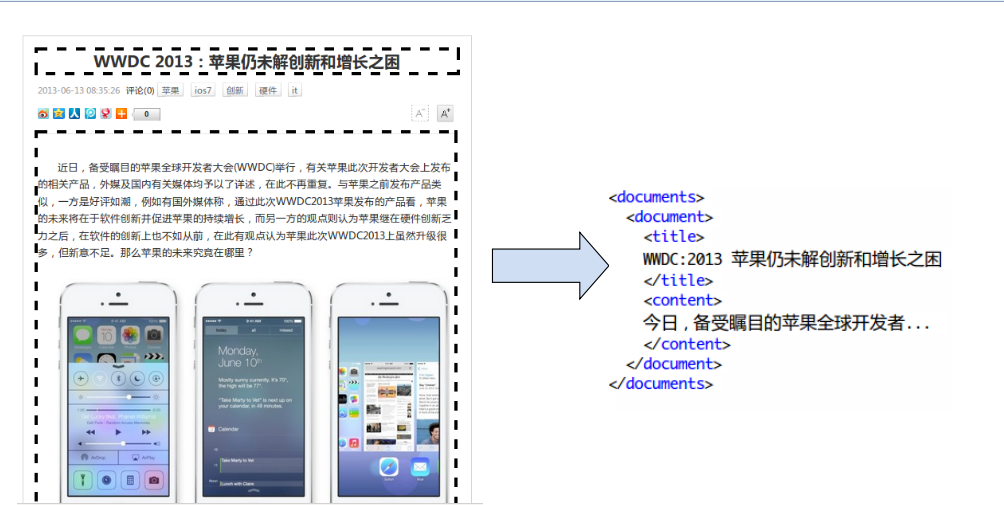
\includegraphics[width=\textwidth]{intro01/news-to-xml}
  \caption{用XML存储新闻的标题和正文示意}
  \label{intro:fig:blog-to-xml}
\end{figure}

\subsection{HTML文档的模板}
\label{sec:htmltemplateintro}
互联网上有成千上万的HTML文档,对于大部分的网站来说,不可能针对每一个网页单独写一
个静态网页存储到服务器。实际上,我们在互联网上浏览的大部分HTML网页都是通过网站的
后台程序动态生成的,只有极少量的还是通过静态HTML方式进行存储。

在Web开发领域,MVC(Model, View, Controller)模式是目前最流行的开发方法。模型
(Model)是对底层数据和业务的进行的封装;视图(View)负责用户界面的交互,包括给用
户发送信息,接受用户输入等;控制器(Controller)则是系统的控制逻辑,对用户请求进
行处理,用选择合适的视图用于显示模型返回的数据。
如\reffig{intro:fig:mvc}所示\footnote{来
  源:http://en.wikipedia.org/wiki/Model\%E2\%80\%93view\%E2\%80\%93controller}。
目前有很多基于MVC模式的Web开发框架,比如基于Ruby语言的Ruby on Rails,基于Python语
言的Django以及基于Scala语言的Play! Framework等等。这些框架用模型对底层的数据库进
行包装,当用户请求一个HTML页面的时候,控制器负责从数据库中查询相应数据,然后在视
图层选择合适的渲染模板,将对应的数据填充到模板中,从而生成目标HTML文档,将其返回
给用户。\reffig{intro:fig:django}是一个简单的用Django开发网站时视图层的模板示例,
其中\texttt{news.title}和\texttt{news.content}是从数据库中得到的查询结果。
\begin{figure}
  \begin{minipage}[t]{0.5\linewidth}
  \centering
  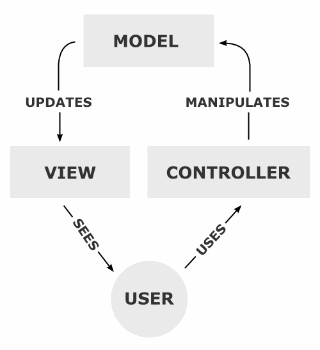
\includegraphics[width=0.8\textwidth]{intro01/MVC-Process}
  \caption{MVC模式}
  \label{intro:fig:mvc}
  \end{minipage}
  \begin{minipage}[t]{0.5\linewidth}
  \centering
  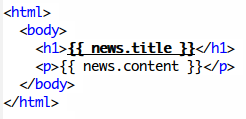
\includegraphics[width=0.8\textwidth]{intro01/django}
  \caption{Django中的HTML模板示例}
  \label{intro:fig:django}
  \end{minipage}
\end{figure}

我们注意到,大部分HTML网页都是通过这种查询底层数据库得到相应数据,然后使用模板进
行渲染的方法生成的。对于大量的从同一个模板生成的网页来说,“模板”就是这些网页
的“公共部分”。实际上,模板的定义要比这里所说的网页的“公共部分”要复杂一些,许
多Web开发框架的模板引擎都支持一些简单的控制结构(如if,for等),如果生成模板的时
候使用了这些控制逻辑,对应的模板也会比较复杂,如\reffig{intro:fig:django-hard}所
示。我们在第~\ref{chap:template}章中将会给出一个较为严格的定义,这里我们先使用这
种直观的定义便于理解。如果我们能够从大量的由同一个模板生成的网页中将它们的模板抽
取出来,那么我们就可以用抽取出来的模板对其他的由同一个模板生成的网页进行内容的抽
取。简单来说,有了网页的模板以后,每个网页中非“模板”的部分即可以认为是通过查询
后台数据库得到的数据动态生成的,而这些数据正是我们所需要提取出来的。
\begin{figure}
  \centering
  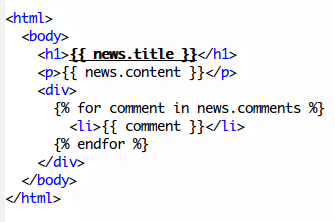
\includegraphics[width=0.5\textwidth]{intro01/django-hard}
  \caption{使用了for的Django模板示例}
  \label{intro:fig:django-hard}
\end{figure}
\section{本文的主要工作}
\label{sec:mainwork}
本文的主要工作是从已经抓取的大量的网页数据中,自动地对其中的网页进行聚类,得到不
同的类别。对于其中的每一类,将其中可能的模板抽取出来,然后再利用这些模板去抽取新
抓取的网页。由于我们的数据量比较大,因此需要设计一些高效的算法进行抽取;同时,海
量数据也提供了较多的冗余性,使得其中一些隐藏的模式和信息可以更好地被挖掘出来,得
到比较好的实验结果。

一个HTML文档由标签和标签所包含的内容所组成。如果仅考虑标签的话,可以根据标签和标
签之间相互的嵌套关系定义一颗仅由标签所组成的树,我们将这样的一棵树称为HTML文档的
结构特征。与之类似,HTML文档中所包含的除标签以外的内容我们称之为HTML文档的内容特
征。参考第~\ref{sec:htmltemplateintro}节所所述的网站后台利用模板生成网页过程,我
们认为模板实际上决定了生成的HTML文档结构特征中最主要的一部分(不是全部),而通过
查询后台数据库中得到的结果动态生成的部分则主要决定了HTML文档的内容特征。按照这种
理解,由同一模板生成的网页将会有较高的结构相似度,而不一定有很高的内容相似度——因
为后台数据库中存储的数据本身没有很大的联系。因此,本文将重点放在了考察HTML文档的
结构特征上,而对文档的内容特征不做太多关注。

互联网上有大量的网站,每个网站的网页都可能采用不同的模板生成。实际上,即使对于同
一个网站,也可能有多个不同的模板。因此,我们需要先对这些网页数据进行聚类,使得同
一个模板生成的网页位于同一类中,便于后续的模板提取。

在模板表示和提取方面,我们将通过寻找结构相似网页中共同的结构特征提取出模板,并利
用提取出的模板对其他网页进行信息抽取。我们希望可以提取出类似
于\reffig{intro:fig:django}中一样的模板,其中动态生成的部分(对
于\reffig{intro:fig:django}来说,即\texttt{\{\{\}\}}中包含的Python表达式)我们用
正则表达式\texttt{.*}代替。
\section{相关工作}
\label{sec:relatedwork}

\subsection{网页结构相似度计算}
\label{sec:relatedwork:sim}
网页的结构特征相似度是我们进行聚类时的标准,因此快速准确地计算出网页的结构相似度
是我们整个工作中非常重要的一部分。在这方面,已经有很多的相关的研究工作。

早期的工作主要集中在HTML文档解析成的DOM Tree上,主要的度量方法是树编辑距离(Tree
Edit Distance)。Tai和Kuo-Chung在\onlinecite{tai1979tree}中提出了计算树编辑距离的
方法,Reis等在\onlinecite{reisauto}中说明了如何利用树编辑距离的方法自动抽取网页新
闻。此外,还有一些优化树编辑距离计算时间的尝试,包括\onlinecite{zhang1989simple,
  dubiner1994faster,touzet2005linear}等。树编辑距离的主要缺点是算法非常复杂,计算
复杂度很高,有些时间上的优化的算法又依赖于各种各样的限制条件。由于我们要处理的数
据量较大,采用复杂度很高树编辑距离算法进行计算是不现实的。

Gottron在\onlinecite{GottronCluster}中介绍了几个基于HTML的标签(tag)集合的计
算HTML文档结构相似度的方法。最简单的一种方法是计算两个HTML文档$D_i,D_{j}$的标签集
合$T_i, T_j$的Jaccard相似度,即
\[
Sim(D_i,D_j)=\frac{|T_i \cap T_j|}{|T_i \cup T_j|}
\]
这种方法在HTML文档上很难取得比较好的效果,因为HTML文档的标签集合是有限的,因此考
察标签集合的Jaccard相似度很难体现不同的模板生成的HTML文档之间的区别。另一种简单的
方法是标签矢量法,即将标签转化为矢量$\vc{V_i}$,每个标签出现次数$N_{t_i}$对应矢
量$\vc{V_i}$的一个分量,然后计算两个矢量的欧几里得距离,得到文档的相似度。
\[
Sim(D_i,D_j)=|\vc{V_i}-\vc{V_j}|
\]
这种方法的缺点是仍然没有考虑标签之间的嵌套关系,只考虑了标签的数量关系,因此丢失
了很多HTML文档结构上的信息。比较好的一种方式是通过某种树的遍历方法,得到树$T_i$一
个标签序列$S_i$,然后计算两个标签序列的最长公共子序列(Longest Common Sequence),

由此得到两者的相似度。即
\[
Sim(D_i,D_j)=\frac{|lcs(S_i,S_j)|}{max(|S_i|,|S_j|)}
\]

还有一类计算相似度的方法是基于路径集合。路径(Path)指的是从根节点到某个目标节点
的标签所组成的序列。Joshi在\onlinecite{joshi2003bag}中提出了利用路径集合来衡量文
档的结构相似度。Buttler等人在\onlinecite{buttler2004short}引入shingle技术,加上一
些随机取样等优化手段,可以在常数时间内计算任意大小的文档之间的相似
度。Kim在\onlinecite{KimText}基于路径集合提出了一种以最小描述距离(Minimum
Description Length)为优化目标、通过Minhash加快计算速度的计算方法。基于路径集合的
方法将HTML的树形结构的相似度转化为序列集合的相似度,序列中标签的顺序仍然保留了原
始DOM Tree的一些层次信息。这种方法与计算树编辑距离的方法相比,在不损失太多的结构
信息的同时有效降低了复杂度,并且有多种优化的途径,是一种比较好的计算结构相似度的
方法。

Flesca在\onlinecite{fft}中还提出了一种有趣的计算文档相似度的方法。他引入信号处理
领域的快速傅里叶变换(FFT)用于处理文本。具体的方法是将文本的序列看成时序序列,利
用快速傅里叶变换将其变换到频域,然后比较幅度的差别。尽管找不到一个可以与之对应的
合理直观的解释,同时Buttler在\onlinecite{buttler2004short}中做的相关的实验也显示
这种方法的效果不是很好,不过就方法本身来说,还是非常有启发意义的。

在Buttler等人在\onlinecite{buttler2004short}的实验中,还有一个值得注意的结果。虽
然树编辑距离看上去是衡量两个文档结构距离的最好标准,但是在某些实验中却显示树编辑
距离算法在HTML文档的聚类效果上不如一些简单的近似算法,比如加权的标签算法和基于路
径集合的近似算法,而且算法在运行时间上远远大于这些近似算法。

\subsection{模板检测与提取}
\label{sec:relatedwork:template}
在网页模板的检测和提取方面,也有很多的相关的研究成果。典型的无监督的方法是Arasu等
人的\onlinecite{arasu2003extracting}。这篇文章提出了一套模板推导引擎,通过比较不
同网页间的相同点和不同点来自动生成网页模板。这种方法的特点是没有语义信息,需要人
工后期指定相关的语义。

半监督的方法则往往同bootstrapping相结
合。Calson在\onlinecite{carlson2008bootstrapping}中,利用部分树对齐(partial
tree alignment)的方式先对网页结构进行对齐,然后利用一些语义特征,对相似度进行打
分,训练模型的时候采用了bootstrapping,减小了标注的工作量。这种方法的缺点是算法运
行速度较慢,不适用于数据量较大的情况。

还有一些工作并没有直接在HTML文档的DOM Tree的层次上进行,而是采用更符合人直观的网
页视觉分块作为基础进行模板提取。Cai等人在\onlinecite{cai2003vips}中提出一种利
用HTML标签的视觉属性信息来检测网页中的视觉分块的方法。这种方法的计算方法比较复杂,
而且目前主流的网页都已采用HTML+CSS架构,原文中布局信息的计算也需要做较大的修改。
\section{本章总结}
\label{sec:summaryintro}
本章最开始主要简单介绍了大数据的研究背景、结构化数据和HTML文档的模板。接着对本文
的主要工作进行了概述,简单说明了我们将在模板聚类和抽取的过程中主要考虑HTML文档的
结构信息。最后我们对网页结构相似度计算和网页模板提取方面已有的研究工作进行了总结
和回顾。

接下来的几章将按以下方式组织:

第二章主要介绍系统的整体框架以及每个模块对应的设计,主要包括预处理模块、网页聚类
模块、模板生成和内容提取模块。

第三章主要介绍预处理模块中如何对HTML文档的重复记录进行检测。这一步主要利用到了后
缀树的数据结构,我们将在这一章中详细介绍基于后缀树的重复记录的检测算法。

第四章主要介绍网页聚类模块的实现。我们以最长公共子序列为基础计算网页的结构相似度,
然后利用层次聚类算法进行聚类。

第五章主要介绍网页模板生成和内容的提取。我们将在之前的聚类结果和最长公共子序列算法
的基础上提出一种无监督的模板生成算法,用于内容的提取。

第六章介绍系统的具体实现细节以及实验的设定和结果。

第七章总结工作,对未来进行展望,提出改进和努力的方向。

%%% Local Variables: 
%%% mode: latex
%%% TeX-master: "../main"
%%% End: 

